\begin{figure}[h!]
	\centering
	
	
	
	\tikzset{every picture/.style={line width=0.75pt}} %set default line width to 0.75pt        
	
	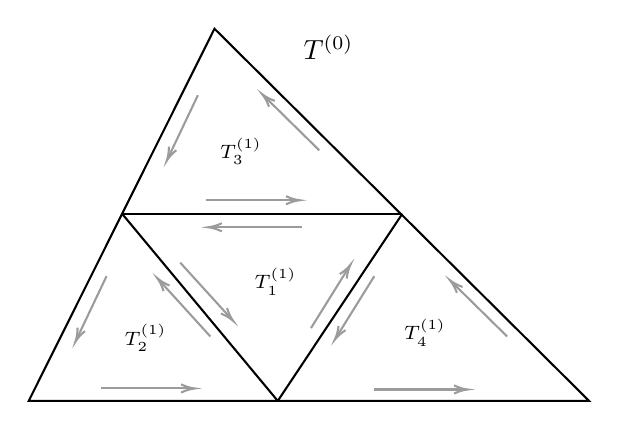
\begin{tikzpicture}[x=0.75pt,y=0.75pt,yscale=-1,xscale=1]
		%uncomment if require: \path (0,300); %set diagram left start at 0, and has height of 300
		
		%Shape: Triangle [id:dp22929948430382896] 
		\draw   (199.5,70.67) -- (380,250) -- (110,250) -- cycle ;
		%Straight Lines [id:da244981817401549] 
		\draw    (155,159.83) -- (290,159.83) ;
		%Straight Lines [id:da07991899539465663] 
		\draw    (155,159.83) -- (230,250) ;
		%Straight Lines [id:da21358766614612867] 
		\draw    (290,159.83) -- (230,250) ;
		%Straight Lines [id:da6197653203930451] 
		\draw [color={rgb, 255:red, 155; green, 155; blue, 155 }  ,draw opacity=1 ]   (195.5,153.32) -- (238.5,153.32) ;
		\draw [shift={(240.5,153.32)}, rotate = 180] [color={rgb, 255:red, 155; green, 155; blue, 155 }  ,draw opacity=1 ][line width=0.75]    (6.56,-1.97) .. controls (4.17,-0.84) and (1.99,-0.18) .. (0,0) .. controls (1.99,0.18) and (4.17,0.84) .. (6.56,1.97)   ;
		%Straight Lines [id:da5794917403292845] 
		\draw [color={rgb, 255:red, 155; green, 155; blue, 155 }  ,draw opacity=1 ]   (250,129.28) -- (223.93,103.63) ;
		\draw [shift={(222.5,102.23)}, rotate = 44.53] [color={rgb, 255:red, 155; green, 155; blue, 155 }  ,draw opacity=1 ][line width=0.75]    (6.56,-1.97) .. controls (4.17,-0.84) and (1.99,-0.18) .. (0,0) .. controls (1.99,0.18) and (4.17,0.84) .. (6.56,1.97)   ;
		%Straight Lines [id:da14151133839867325] 
		\draw [color={rgb, 255:red, 155; green, 155; blue, 155 }  ,draw opacity=1 ]   (191.5,102.73) -- (177.36,132.48) ;
		\draw [shift={(176.5,134.28)}, rotate = 295.42] [color={rgb, 255:red, 155; green, 155; blue, 155 }  ,draw opacity=1 ][line width=0.75]    (6.56,-1.97) .. controls (4.17,-0.84) and (1.99,-0.18) .. (0,0) .. controls (1.99,0.18) and (4.17,0.84) .. (6.56,1.97)   ;
		%Straight Lines [id:da6438773878089432] 
		\draw [color={rgb, 255:red, 155; green, 155; blue, 155 }  ,draw opacity=1 ]   (147.5,189.89) -- (133.36,219.64) ;
		\draw [shift={(132.5,221.45)}, rotate = 295.42] [color={rgb, 255:red, 155; green, 155; blue, 155 }  ,draw opacity=1 ][line width=0.75]    (6.56,-1.97) .. controls (4.17,-0.84) and (1.99,-0.18) .. (0,0) .. controls (1.99,0.18) and (4.17,0.84) .. (6.56,1.97)   ;
		%Straight Lines [id:da5035255329161727] 
		\draw [color={rgb, 255:red, 155; green, 155; blue, 155 }  ,draw opacity=1 ]   (145,243.99) -- (188,243.99) ;
		\draw [shift={(190,243.99)}, rotate = 180] [color={rgb, 255:red, 155; green, 155; blue, 155 }  ,draw opacity=1 ][line width=0.75]    (6.56,-1.97) .. controls (4.17,-0.84) and (1.99,-0.18) .. (0,0) .. controls (1.99,0.18) and (4.17,0.84) .. (6.56,1.97)   ;
		%Straight Lines [id:da20703213743187354] 
		\draw [color={rgb, 255:red, 155; green, 155; blue, 155 }  ,draw opacity=1 ]   (197.5,218.94) -- (173.35,192.37) ;
		\draw [shift={(172,190.89)}, rotate = 47.73] [color={rgb, 255:red, 155; green, 155; blue, 155 }  ,draw opacity=1 ][line width=0.75]    (6.56,-1.97) .. controls (4.17,-0.84) and (1.99,-0.18) .. (0,0) .. controls (1.99,0.18) and (4.17,0.84) .. (6.56,1.97)   ;
		%Straight Lines [id:da8174786530331881] 
		\draw [color={rgb, 255:red, 155; green, 155; blue, 155 }  ,draw opacity=1 ]   (340.5,218.94) -- (314.43,193.29) ;
		\draw [shift={(313,191.89)}, rotate = 44.53] [color={rgb, 255:red, 155; green, 155; blue, 155 }  ,draw opacity=1 ][line width=0.75]    (6.56,-1.97) .. controls (4.17,-0.84) and (1.99,-0.18) .. (0,0) .. controls (1.99,0.18) and (4.17,0.84) .. (6.56,1.97)   ;
		%Straight Lines [id:da7674415762467801] 
		\draw [color={rgb, 255:red, 155; green, 155; blue, 155 }  ,draw opacity=1 ]   (276.5,244.49) -- (319.5,244.49) ;
		\draw [shift={(321.5,244.49)}, rotate = 180] [color={rgb, 255:red, 155; green, 155; blue, 155 }  ,draw opacity=1 ][line width=0.75]    (6.56,-1.97) .. controls (4.17,-0.84) and (1.99,-0.18) .. (0,0) .. controls (1.99,0.18) and (4.17,0.84) .. (6.56,1.97)   ;
		%Straight Lines [id:da06674836216123325] 
		\draw [color={rgb, 255:red, 155; green, 155; blue, 155 }  ,draw opacity=1 ]   (276.5,189.89) -- (258.56,218.75) ;
		\draw [shift={(257.5,220.45)}, rotate = 301.87] [color={rgb, 255:red, 155; green, 155; blue, 155 }  ,draw opacity=1 ][line width=0.75]    (6.56,-1.97) .. controls (4.17,-0.84) and (1.99,-0.18) .. (0,0) .. controls (1.99,0.18) and (4.17,0.84) .. (6.56,1.97)   ;
		%Straight Lines [id:da5880950101661566] 
		\draw [color={rgb, 255:red, 155; green, 155; blue, 155 }  ,draw opacity=1 ]   (198.5,166.34) -- (241.5,166.34) ;
		\draw [shift={(196.5,166.34)}, rotate = 0] [color={rgb, 255:red, 155; green, 155; blue, 155 }  ,draw opacity=1 ][line width=0.75]    (6.56,-1.97) .. controls (4.17,-0.84) and (1.99,-0.18) .. (0,0) .. controls (1.99,0.18) and (4.17,0.84) .. (6.56,1.97)   ;
		%Straight Lines [id:da10416251901852114] 
		\draw [color={rgb, 255:red, 155; green, 155; blue, 155 }  ,draw opacity=1 ]   (207.15,209.95) -- (183,183.38) ;
		\draw [shift={(208.5,211.43)}, rotate = 227.73] [color={rgb, 255:red, 155; green, 155; blue, 155 }  ,draw opacity=1 ][line width=0.75]    (6.56,-1.97) .. controls (4.17,-0.84) and (1.99,-0.18) .. (0,0) .. controls (1.99,0.18) and (4.17,0.84) .. (6.56,1.97)   ;
		%Straight Lines [id:da2685827787461035] 
		\draw [color={rgb, 255:red, 155; green, 155; blue, 155 }  ,draw opacity=1 ]   (263.94,186.08) -- (246,214.93) ;
		\draw [shift={(265,184.38)}, rotate = 121.87] [color={rgb, 255:red, 155; green, 155; blue, 155 }  ,draw opacity=1 ][line width=0.75]    (6.56,-1.97) .. controls (4.17,-0.84) and (1.99,-0.18) .. (0,0) .. controls (1.99,0.18) and (4.17,0.84) .. (6.56,1.97)   ;
		
		% Text Node
		\draw (217.33,184.4) node [anchor=north west][inner sep=0.75pt]  [font=\scriptsize]  {$T_{1}^{( 1)}$};
		% Text Node
		\draw (154.67,211.73) node [anchor=north west][inner sep=0.75pt]  [font=\scriptsize]  {$T_{2}^{( 1)}$};
		% Text Node
		\draw (200.67,121.73) node [anchor=north west][inner sep=0.75pt]  [font=\scriptsize]  {$T_{3}^{( 1)}$};
		% Text Node
		\draw (289.33,209.07) node [anchor=north west][inner sep=0.75pt]  [font=\scriptsize]  {$T_{4}^{( 1)}$};
		% Text Node
		\draw (241,72.4) node [anchor=north west][inner sep=0.75pt]    {$T^{( 0)}$};
		
		
	\end{tikzpicture}
\end{figure}